\section{Additional results}
\label{app:additional-results}

\emph{Optional appendix: include only supplementary material needed to support
the explanation. Keep the results required to answer tasks 1--10 in the main report.}

% Delete figures that do not add evidence beyond the main text/tables.
\begin{figure}[htbp]
    \centering
    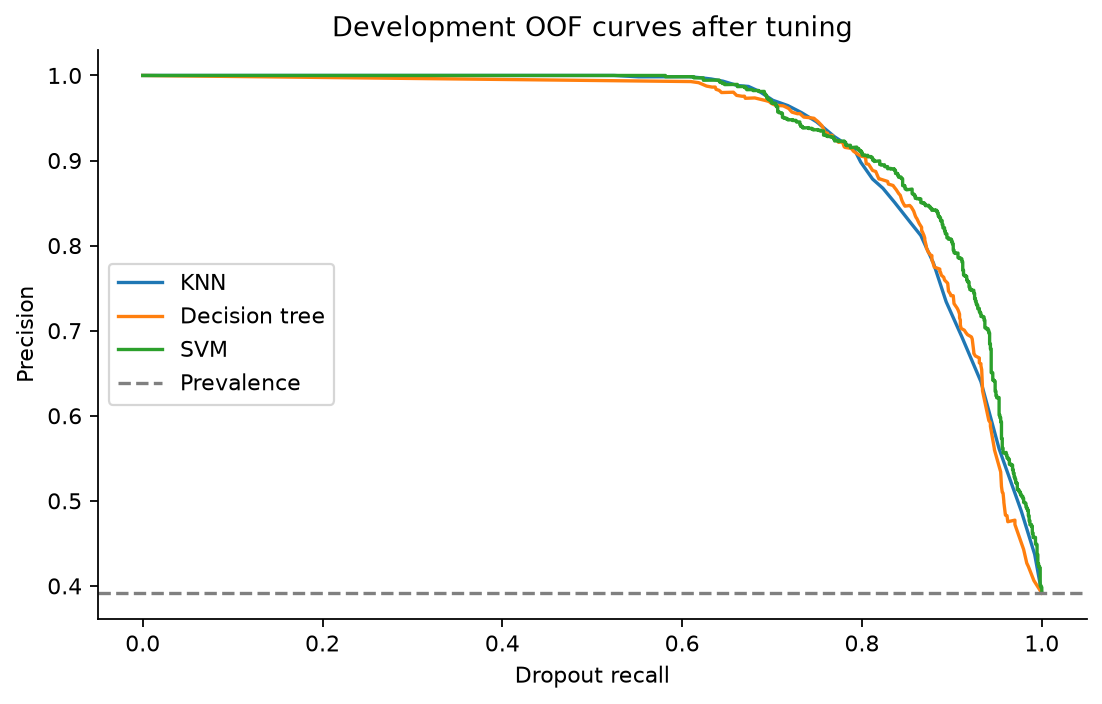
\includegraphics[width=0.8\linewidth]{Images/02_basic_development_pr.png}
    \caption{Development out-of-fold PR curves after tuning; the development
    observations were also used for model selection.}
    \label{fig:basic-development-pr}
\end{figure}

\begin{figure}[htbp]
    \centering
    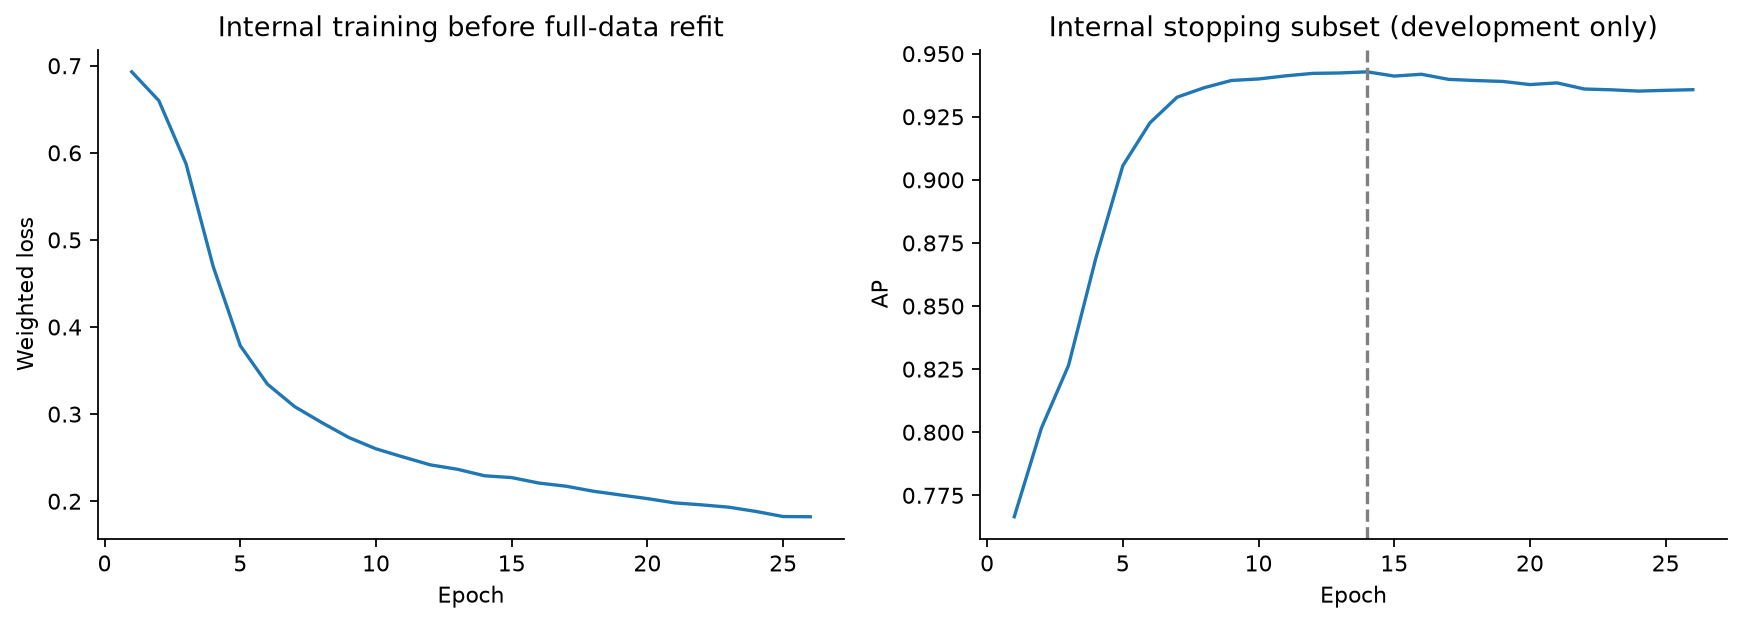
\includegraphics[width=\linewidth]{Images/03_deep_network_learning.png}
    \caption{Internal loss and stopping-subset AP used to choose the epoch count
    before the fresh full-development fit.}
    \label{fig:deep-network-learning}
\end{figure}

\begin{figure}[htbp]
    \centering
    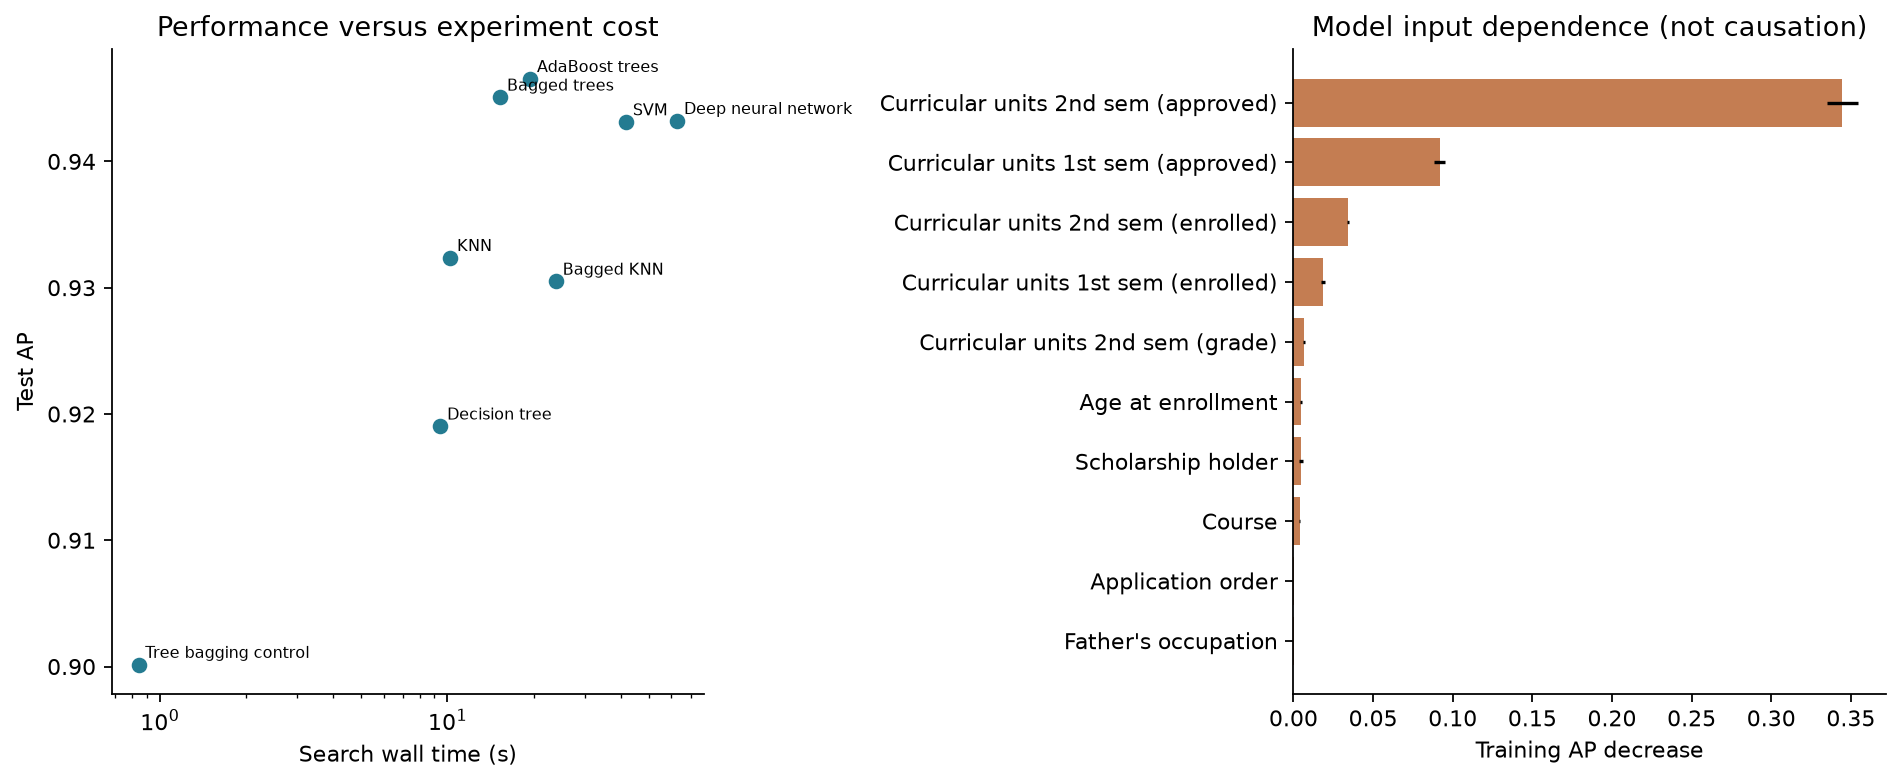
\includegraphics[width=\linewidth]{Images/05_cost_and_input_dependence.png}
    \caption{Search cost versus held-out AP and training permutation dependence.
    Input dependence does not establish causation.}
    \label{fig:cost-input-dependence}
\end{figure}

\begin{figure}[htbp]
    \centering
    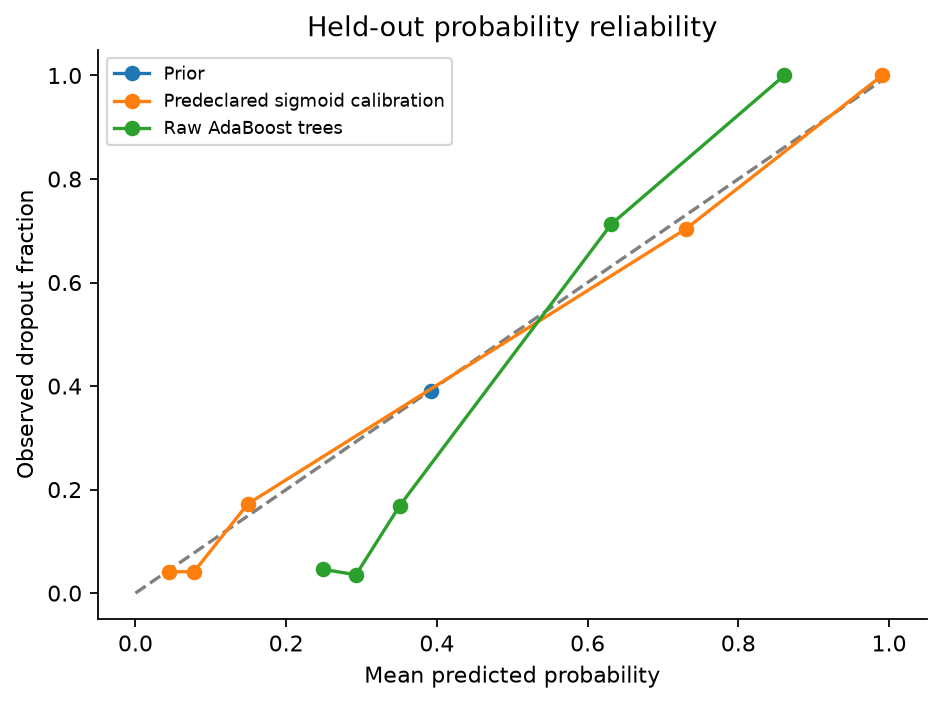
\includegraphics[width=0.75\linewidth]{Images/06_probability_reliability.png}
    \caption{Held-out reliability for the raw workflow, its predeclared
    sigmoid-calibrated variant and the training prior.}
    \label{fig:probability-reliability}
\end{figure}
